
\section{Cálculo}
\subsection{Teoría}
\subsubsection{Longitud de arco en coordenadas cartesianas}


%%%%%%%%%%%%%%%%%%%%%%%
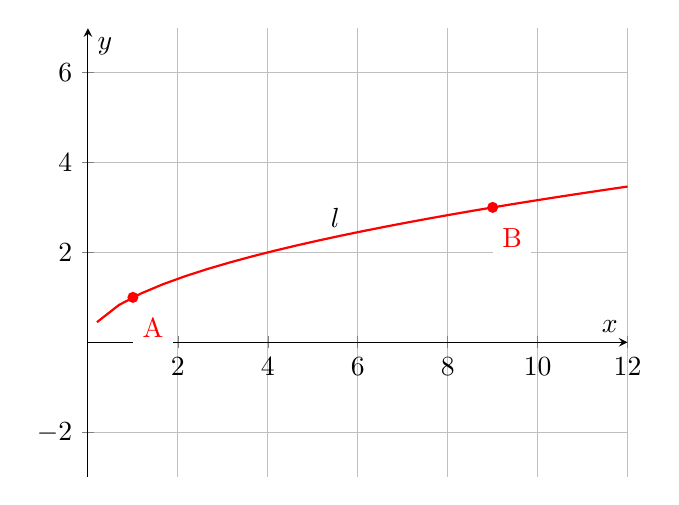
\begin{tikzpicture}
\begin{axis}[axis lines=middle,axis equal, grid=both, xlabel=$x$,    ylabel=$y$,domain=0.2:12, xmax=12,xmin=0,ymax=4,ymin=0]
\addplot[red,thick] {( x^(0.5)};
\fill[red] (1,1) circle (2pt) node [below right,fill=white,yshift=-4pt] {A};


\fill[red] (9,3) circle (2pt) node [below right,fill=white,yshift=-4pt] {B};
\draw[thick,red] (5.5,2.3453) coordinate (a) ;
\draw (a) node[above] {$l$};

\end{axis}
\end{tikzpicture}
\\Sea $f(x)$ una función continua y derivable.\\
La longitud de arco $l$, está dado por:
\begin{equation*}
l=\int_a^b\sqrt{1+{f'(x)}^2}
\mathrm{d}x=
\end{equation*}